\section{PROFETA}
%------------------------------
\begin{frame}[label=3]{PROFETA}  
\begin{itemize}
   \item 
   \navy{PROFETA} adds logic constructs to Python programs, thus 
    offering an all-in-one environment for both approaches
    \N
  \item
    \navy{PROFETA} exploits the key concepts of the \red{B}elief-\red{D}esire- \red{I}ntention model.
  \end{itemize}
  \N\N
\end{frame}
%------------------------------





%
%%------------------------------
%%\subsection{}
%%------------------------------
%
%



















%
%\begin{frame}{Graph Models}
%  % Image
%  \begin{figure}[!h]
%    \begin{center}
%      \fbox{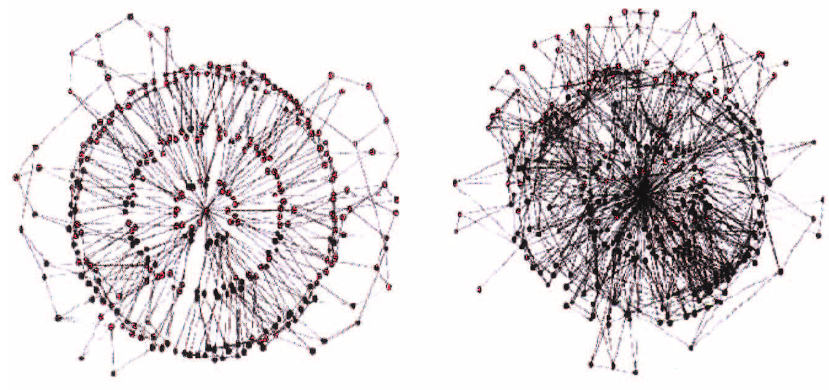
\includegraphics[width=150pt]{img/sample.png}}
%    \end{center}
%  \end{figure}
%\end{frame}
%%
%%
%\begin{frame}{Random Graphs}
%  \begin{itemize}
%    \item Formul\ae\\
%    \item \red{p}$*$\red{$N_1$}$*$(\red{N} - 1) / 2 connections
%  \end{itemize}
%\end{frame}
%%
%%
%\begin{frame}{SampleCode}
%We used the \red{peersim} library\footnote{\tiny{http://peersim.sourceforge.net/}} 
%  \begin{samplecode}
%    \begin{small}
%      // Generate a graph with an average of \red{k} connections\newline
%      // per node and randomness \red{r}\newline
%      Graph g = GraphFactory.wireKOut(g, k, r);\newline
%    \end{small}
%  \end{samplecode}
%\end{frame}
%%
%%
%\begin{frame}{SampleCode2}
%  \begin{samplecode}
%    \begin{tiny}
%      \begin{tabbing}
%        @WebService() \= public class \red{GraphService} \{\\
%        \> @WebMethod() public int [] \red{countNeighbours} (@WebParam() int [] adjVector) \{...\}\\
%        \> @WebMethod() public String [] \red{processConnections} (@WebParam() int [] neighboursCount) \{ ... \}\\
%        \> @WebMethod() \= public int [] \red{computeHops} ( @WebParam() int [] adjVector, \\
%        \> \> @WebParam() int [] neighbourCount,\\
%        \> \> @WebParam() int hyperNodeIndex) \{ ... \}\\
%        \}
%      \end{tabbing}
%    \end{tiny}
%  \end{samplecode}
%\end{frame}
%%
%
